\documentclass[a4paper, fontsize=14pt]{article}
\usepackage[T2A]{fontenc}
\usepackage{mathtools}
\usepackage[utf8]{inputenc}
\usepackage[english, russian]{babel}
\usepackage{fancyhdr}
\usepackage{graphicx}
\usepackage{gensymb}
\usepackage{floatrow}
\usepackage{titlesec}
\usepackage{lastpage}
\usepackage{float}
\usepackage{gensymb}
\usepackage{booktabs}
\usepackage{amsmath}
\usepackage{amssymb}
\usepackage{cmap}

\pagestyle{fancy}
	\fancyhf{}
	\lhead{\hspace{1bp} Работа \textnumero 1.3.3}
	\rhead{Терехов Максим 876\hspace{1bp}}
	\cfoot{\textbf{}}
	\rfoot{\thepage\ \textnormal{из}\ \pageref{LastPage}}
	\renewcommand{\headrulewidth}{1pt}
	\renewcommand{\footrulewidth}{1pt}


%\addtolength{\hoffset}{-1.75cm}
%\addtolength{\textwidth}{3.5cm} 

%\addtolength{\voffset}{-1.5cm}
%\addtolength{\textheight}{3cm} 

\titleformat{\section}
    [block]{\normalfont\bfseries\large}{\rlap{\thesection}}{0em}
    {\vspace{-0.02\textwidth}\begin{minipage}[t]{.95\textwidth}}
[\end{minipage}]

\thispagestyle{fancy}

\begin{document}
\selectlanguage{russian}
\parindent=1cm


\huge
\centering
\textbf{Определение вязкости воздуха по скорости течения через тонкие трубки}

\raggedright
\large
\section*{Цель работы}
Экспериментально выявить участок сформированного течения;
 определить режимы ламинарного и турбулентного течения;
 определить число Рейнольдса.
\section*{Оборудование}
Металлические трубки, укреплённые на горизонтальной подставке; газовый счётчик;
микроманометр типа MMH; стеклянная U-образная трубка; секундомер.
\section*{Экспериментальная установка}
\begin{figure}[H]
\center
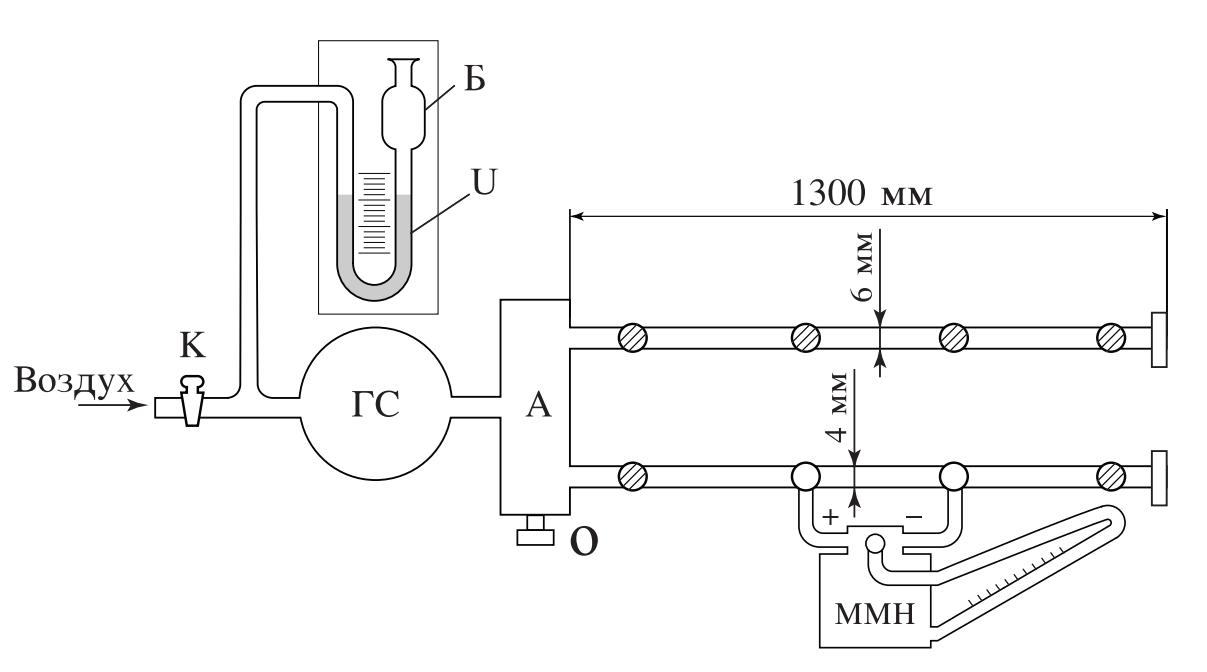
\includegraphics[scale=0.25]{asd.png}
\caption{Схема установки}
\end{figure}

\begin{figure}[H]
\center
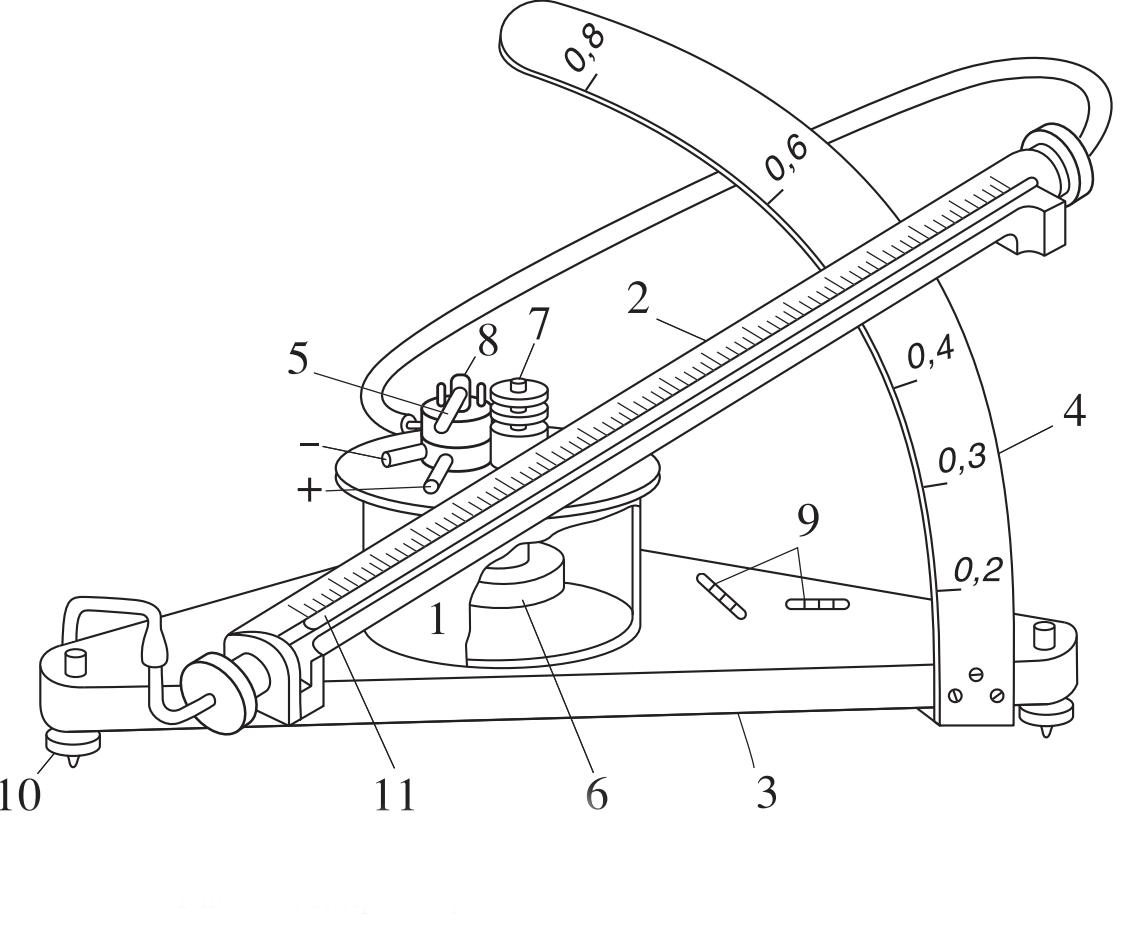
\includegraphics[scale=0.25]{mic.png}
\caption{Подробная схема микроманометра}
\end{figure}
\section*{Теоретическая часть}
Рассмотрим движение вязкой жидкости или газа по трубке круглого сечения. При малых скоростях потока движение оказывается ламинарным (слоистым), скорости частиц меняются по радиусу и направлены вдоль оси трубки. С увеличением скорости потока движение становится турбулентным, а слои перемешиваются. При турбулентном движении скорость в каждой точке быстро меняет величину и направление, сохраняется только средняя величина скорости.

Характер движения газа (или жидкости) в трубке определяется безразмерным числом Рейнольдса:
\[
	Re = \frac{vr\rho}{\eta},
\]
где $v$ --- скорость потока, $r$ --- радиус трубки, $\rho$ --- плотность движущейся среды, $\eta$ --- её вязкость. В гладких трубах круглого сечения переход от ламининарного движения к турбулентному происходит при $Re \approx 1000$.

При ламинарном течении объем газа $V$, протекающий за время $t$ по трубе длиной $l$, определяется формулой Пуазейля:
\begin{equation}
	Q\text{v} = \frac{\pi r^4}{8 l \eta}(P_1 - P_2).
\end{equation}
В этой формуле $P_1 - P_2$ --- разность давлений в двух выбранных сечениях 1 и 2, расстояние между которыми равно $l$. Величину $Q$ обычно называют расходом. Формула (1) позволяет определять вязкость газа по его расходу.

Отметим условия, при которых справедлива формула (1). Прежде всего необходимо, чтобы с достаточным запасом выполнялось неравенство $Re < 1000$. Необходимо также, чтобы при течении не происходило существенного изменения удельного объёма газа (при выводе формулы удельный объём считался постоянным). Для жидкости это предположение выполняется практически всегда, а для газа --- лишь в тех случаях, когда перепад давлений вдоль трубки мал по сравнению с самим давлением. В нашем случае давление газа равно атмосферному ($10^3$ см вод. ст.), а перепад давлений составляет не более 10 см вод. ст., т. е. менее 1\% от атмосферного. Формула (1) выводится для участков трубки, на которых закон распределения скоростей газа по сечению не меняется при двидении вдоль потока.
\begin{figure}[H]
\center
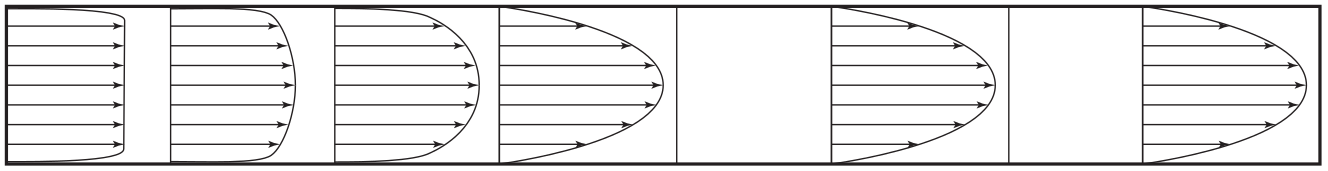
\includegraphics[scale=0.25]{potok.png}
\caption{Формирование потока газа в трубке круглого сечения}
\end{figure}
При втекании газа в трубку из большого резервуара скорости слоёв вначале постоянны по всему направлению. По мере продвижения газа по трубке картина распределения скоростей меняется, так как сила трения о стенку тормозит прилежащие к ней оси. Характерное для ламинарного течения параболическое распределение скоростей устанавливается на некотором расстоянии $a$ от входа в трубку, которое зависит от радиуса трубки $r$ и числа Рейнольдса по формуле 
\begin{equation}
	a \approx 0.2 r \cdot Re.
\end{equation}
Градиент давления на участке формирования потока оказывается б\'{о}льшим, чем на участке с установившимся ламинарным течением, что позволяет разделить эти участки экспериментально. Формула (2) даёт возможность оценить дину участка формирования.
\newpage
\section*{Обработка результатов измерений}
Оценим расстояние, на котором происходит формирование потока при ламинарном течении:
\[
	a \approx 0.2 r \cdot Re = 41\, \text{см}
\]
Давление, измеряемое микроманометром, определяется по формуле:
\[
P=K \cdot l \cdot 9,80665\, \text{Па},
\]
где $P$ --- давление в Паскалях, $l$ --- отчет по шкале, $K=0,2$ --- постоянная угла наклона.
Таблица измерений:\\
\begin{table}[H]

	\centering
	\begin{tabular}{|c|c|c|c|c|c|c|c|c|c|} \hline
  $\Delta V, \, \text{л}$ &   $N$ &   $l,\, \text{мм}$ &     $t_1, c$ &     $t_2, c$ &     $t_3, c$ &     $t_4, c$ &  $ Q, 10^{-3} \frac{\text{л}}{c} $ & $\Delta P, 10^{-3}\, \text{Па}$ \\\hline
  0.5 &   1 &  10 &  42.85 &  42.12 &  42.19 &  41.92 &  11.83 &   19.61 \\\hline
 0.5 &   2 &  15 &  26.12 &  25.80 &  26.03 &  25.79 &  19.28 &   29.42 \\\hline
 1.0 &   3 &  20 &  37.69 &  36.44 &  37.78 &  36.25 &  27.00 &   39.23 \\\hline
  1.0 &   4 &  25 &  29.12 &  28.32 &  28.25 &  29.07 &  34.86 &   49.03 \\\hline
  1.5 &   5 &  30 &  35.69 &  35.29 &  35.81 &  35.63 &  42.13 &   58.84 \\\hline
  1.5 &   6 &  35 &  30.28 &  29.62 &  29.41 &  29.96 &  50.31 &   68.65 \\\hline
  2.0 &   7 &  40 &  35.09 &  35.25 &  35.22 &  35.28 &  56.80 &   78.45 \\\hline
  2.0 &   8 &  45 &  30.59 &  30.75 &  30.71 &  30.41 &  65.33 &   88.26 \\\hline
  2.5 &   9 &  50 &  34.78 &  34.55 &  34.52 &  34.49 &  72.29 &   98.07 \\\hline
  2.5 &  10 &  60 &  30.02 &  30.08 &  29.45 &  29.92 &  83.70 &  117.68 \\\hline
  3.0 &  11 &  65 &  33.56 &  33.72 &  33.49 &  33.49 &  89.38 &  127.49 \\\hline
  3.0 &  12 &  70 &  32.25 &  32.10 &  32.12 &  32.17 &  93.28 &  137.29 \\\hline
  3.0 &  13 &  75 &  31.55 &  31.29 &  31.36 &  31.30 &  95.62 &  147.10 \\\hline
\end{tabular}
		\caption{Измерения на первой трубке}
\end{table}


Построим график зависимости давления от расхода:
\begin{figure}[H]
\center
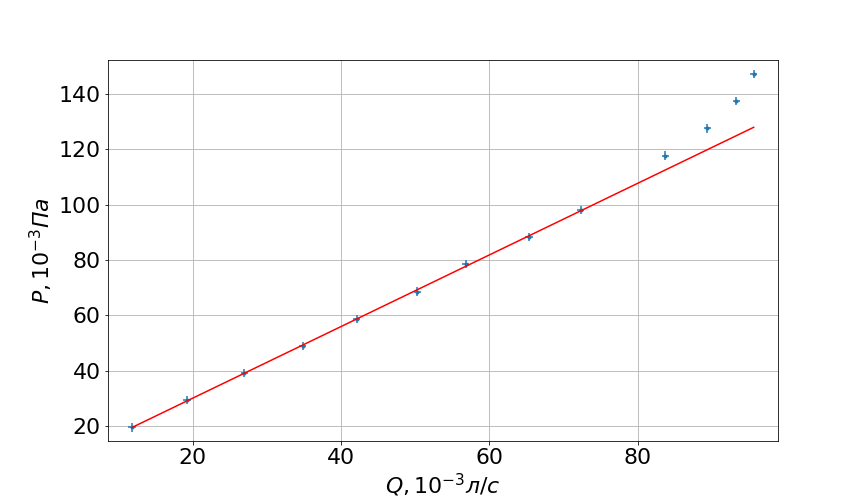
\includegraphics[scale=0.39]{PQ.png}
\caption{Зависимость расхода от разности давлений}
\end{figure}

Коэффициент угла наклона графика: $k = 1.293 \cdot 10^{3} \frac{\text{Па} \cdot c}{\text{м}^3}$

Искомая вязкость:
\[
	\eta = \frac{\pi r^4 k}{8 l} = (17.6 \pm 0.9) \cdot 10^{-6} \text{Па} \cdot \text{c}
\]
Из графика видно, что ламинарный режим переходит в турбулентный на значениях $Q \approx 80 \cdot 10^{-6} \frac{\text{м}^3}{c}$
Посчитаем число Рейнольдса:
\[
	Re = \frac{vr\rho}{\eta} = 	\frac{Q \rho}{\pi r \eta} \approx  850
\]

Построим график зависимости отношения давления от расстояния:
\begin{figure}[H]
\center
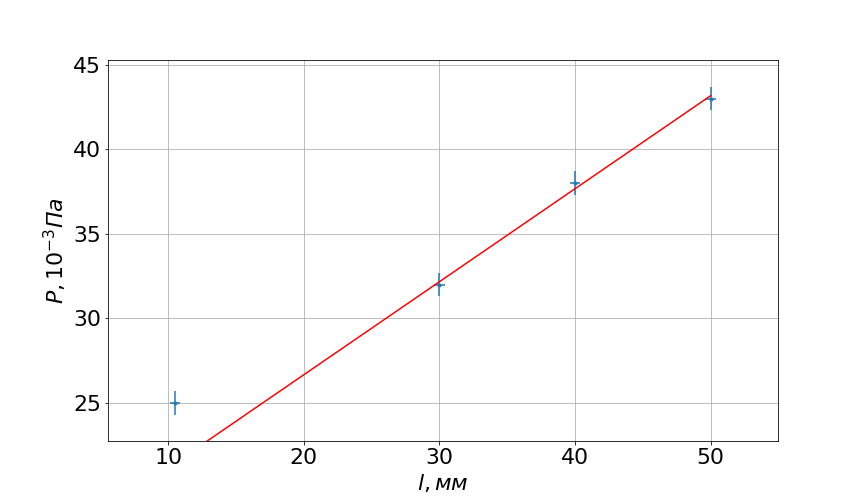
\includegraphics[scale=0.4]{Pl.png}
\end{figure}
Из графика видно, что установление потока происходит примерно на расстоянии 15 см. Теоретическое значение $a \approx 0.2 r Re \approx 35 \text{см}$. То есть оценка, полученная по формуле, гораздо более грубая, чем результат, который мы наблюдаем в эксперименте.

Оценим показатель степени радиуса в формуле Пуазейля:
 
 \begin{table}[H]
 	\centering
 	\begin{tabular}{|c|c|c|c|c|c|c|c|c|} \hline
  $\Delta V, \, \text{л}$ &   $N$ &   $l,\, \text{мм}$ &     $t_1, c$ &     $t_2, c$ &     $t_3, c$ &     $t_4, c$ &  $ Q, 10^{-3} \frac{\text{л}}{c} $ & $\Delta P, 10^{-3}\, \text{Па}$ \\\hline
  2 &  1 &  10 &  31.90 &  32.00 &  32.00 &  31.98 &   62.56 &  19.61 \\\hline
  2 &  2 &  15 &  21.32 &  21.42 &  21.38 &  21.23 &   93.73 &  29.42 \\\hline
  5 &  3 &  20 &  40.44 &  40.69 &  40.41 &  40.57 &  123.37 &  39.23 \\\hline
  5 &  4 &  25 &  34.91 &  35.19 &  35.09 &  35.02 &  142.64 &  49.03 \\\hline
  5 &  5 &  30 &  32.91 &  32.97 &  33.06 &  32.95 &  151.64 &  58.84 \\\hline
  5 &  6 &  35 &  31.38 &  31.40 &  31.47 &  31.47 &  159.08 &  68.65 \\\hline
	\end{tabular}
	\caption{Измерения по второй трубке}

 \end{table}
 \begin{figure}[H]
\center
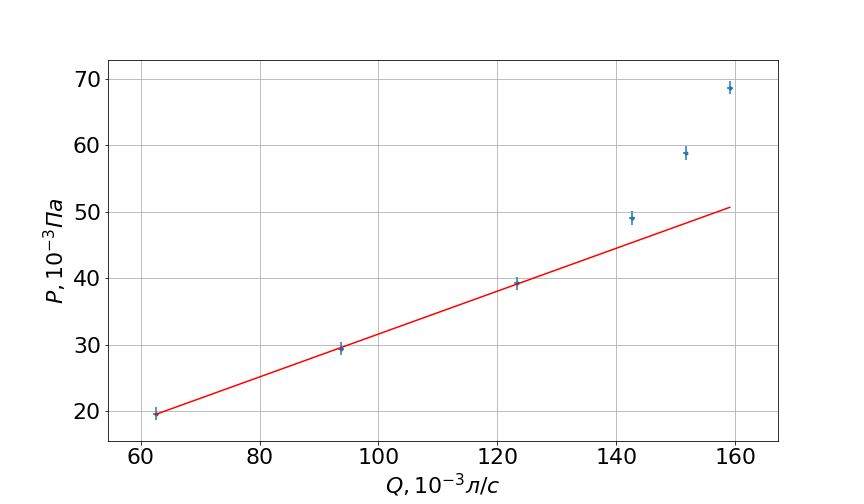
\includegraphics[scale=0.4]{PQ2.png}
\caption{Зависимость расхода от разности давлений}
\end{figure}

Коэффициент угла наклона графика: $k = 0.622 \cdot 10^{3} \frac{\text{Па} \cdot c}{\text{м}^3}$
 
Построим график зависимости $\ln(8l\eta Q/\pi \Delta P)\ \text{от}\ \ln(r))$:
\begin{figure}[H]
\center
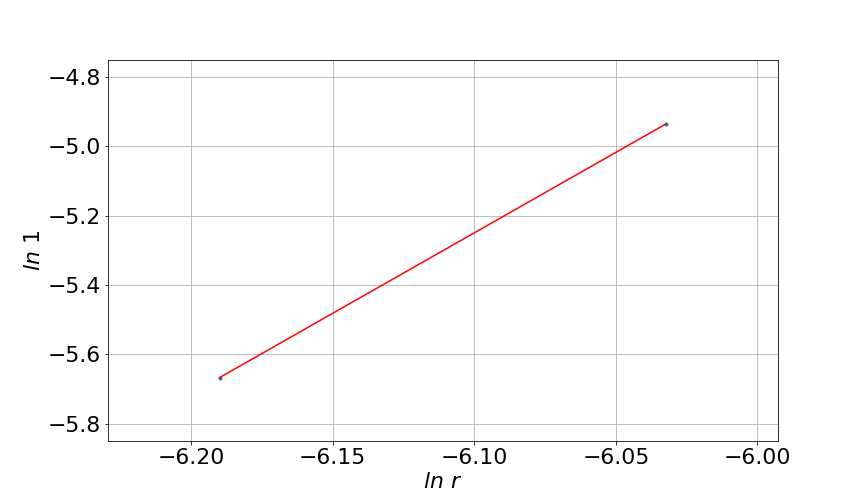
\includegraphics[scale=0.4]{result.png}
\end{figure}

\[
	n = 4.64
\]
Мы получили значение, которое немного отличается от теоретического из формулы Пуазейля, потому что для его нахождения было использовано всего 2 точки.
\newpage
\section*{Вывод}
Полученным методом с использованием формулы Пуазейля мы получили значение вязкости $\eta =  (17.6 \pm 0.9) \cdot 10^{-6}\ \text{Па} \cdot \text{c}$, которое совпадает с учетом погрешности с табличным при этой температуре: $\eta_\text{табл} = 18.4 \cdot 10^{-6} \ \text{Па} \cdot \text{c}$
\end{document}
